\documentclass[tikz,border=5pt]{standalone}
\usepackage{fontspec}
\setmainfont{Times New Roman}
\usepackage{unicode-math}
\setmathfont{Cambria Math}
\usetikzlibrary{shapes.geometric,positioning,fit,backgrounds,arrows.meta,calc}

\begin{document}
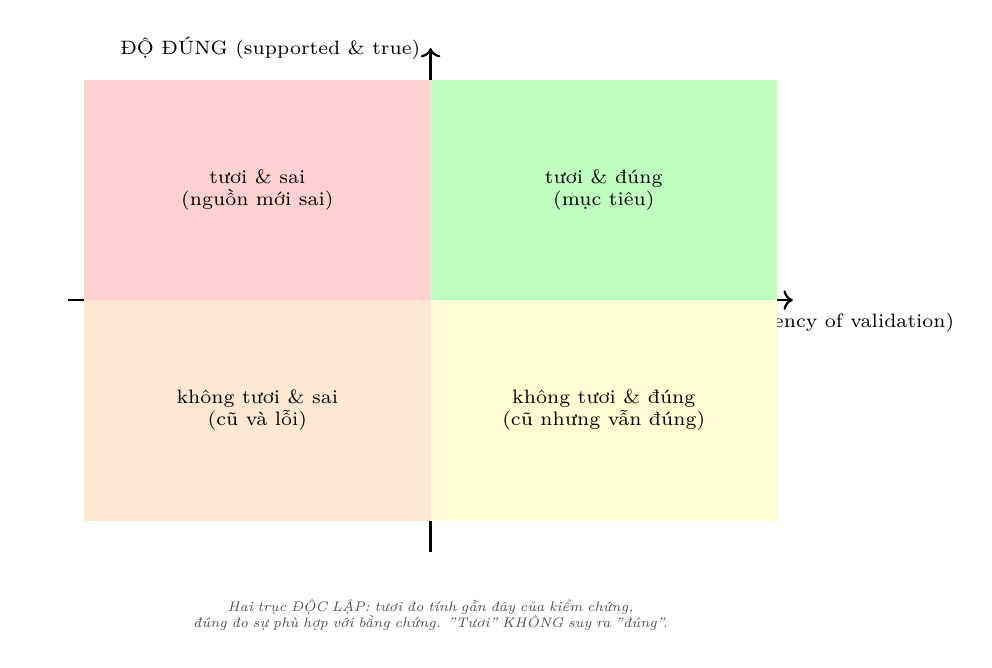
\begin{tikzpicture}[
  arrow/.style={-{Stealth[length=2.2mm]}, thick},
  label/.style={font=\tiny\itshape, text=gray!60!black},
]

% === FRESHNESS vs CORRECTNESS AXES ===
\draw[->, thick] (-4.6, 0) -- (4.6, 0) node[below, font=\scriptsize] {ĐỘ TƯƠI (recency of validation)};
\draw[->, thick] (0, -3.2) -- (0, 3.2) node[left, font=\scriptsize] {ĐỘ ĐÚNG (supported \& true)};

\fill[green!25] (0,0) rectangle (4.4,2.8);
\fill[red!18] (-4.4,0) rectangle (0,2.8);
\fill[orange!18] (-4.4,-2.8) rectangle (0,0);
\fill[yellow!18] (0,-2.8) rectangle (4.4,0);

\node[font=\scriptsize, align=center] at (2.2, 1.4) {tươi \& đúng\\(mục tiêu)} ;
\node[font=\scriptsize, align=center] at (-2.2, 1.4) {tươi \& sai\\(nguồn mới sai)} ;
\node[font=\scriptsize, align=center] at (-2.2, -1.4) {không tươi \& sai\\(cũ và lỗi)} ;
\node[font=\scriptsize, align=center] at (2.2, -1.4) {không tươi \& đúng\\(cũ nhưng vẫn đúng)} ;

\node[label, align=center, text width=10cm] at (0, -4.0)
  {Hai trục ĐỘC LẬP: tươi đo tính gần đây của kiểm chứng,\\đúng đo sự phù hợp với bằng chứng. "Tươi" KHÔNG suy ra "đúng".};
\end{tikzpicture}
\end{document}